
%% for nicer tables
\setlength{\doublerulesep}{\arrayrulewidth}



\section{Transporting data}
\label{sec:transporting}

A very basic problem that keeps cropping up in robotics projects is
simply how to move data around between sensors, processors,
and actuators.  There's a universe of ``middleware'' solutions
in existence for communication (see the survey in \cite{kramer2007development}
and the related-work review in \cite{collett2005player}).
%
%
%
Our own preferred solution
in YARP has the following features:

\begin{itemize} \pflist

\item We use an abstract model of communication that is
transport-neutral and peer-to-peer.

\item The underlying transport used for each individual connection
between peers can be selected independently.  Choices such as network
versus shared memory, tcp versus udp, unicast versus multicast, text
versus binary, which of several networks to transmit on, etc can be
made on a case by case basis.  We encourage such details to be
external configuration choices rather than properties embedded in
programs.

\item We are careful to have one text-mode transport that is
extremely easy to implement, for those who wish to interact with a
YARP system without using any of the YARP libraries or executables.
We believe this is very important for supporting interoperability, and
providing a gentle slope to integrating YARP into an existing system
or vice versa.

\item The model of communication is not intertwined with our
ideas about how devices work or how processes should be started/stopped.
Thus users can ``cherry-pick'' the parts that work for them.

\end{itemize}

Communication in YARP generally follows the {\it Observer} design
pattern. Special port\footnote{
Don't confuse YARP ports with TCP/IP socket port numbers.
We use the word 
``port'' to refer to the former and ``port number'' to refer to the latter.
} objects deliver messages to any number of
observers (other ports), in any number of processes, distributed
across any number of machines, using any of several underlying
communication protocols.





\subsection{The YARP Network}


\begin{figure}[t]
\centerline{
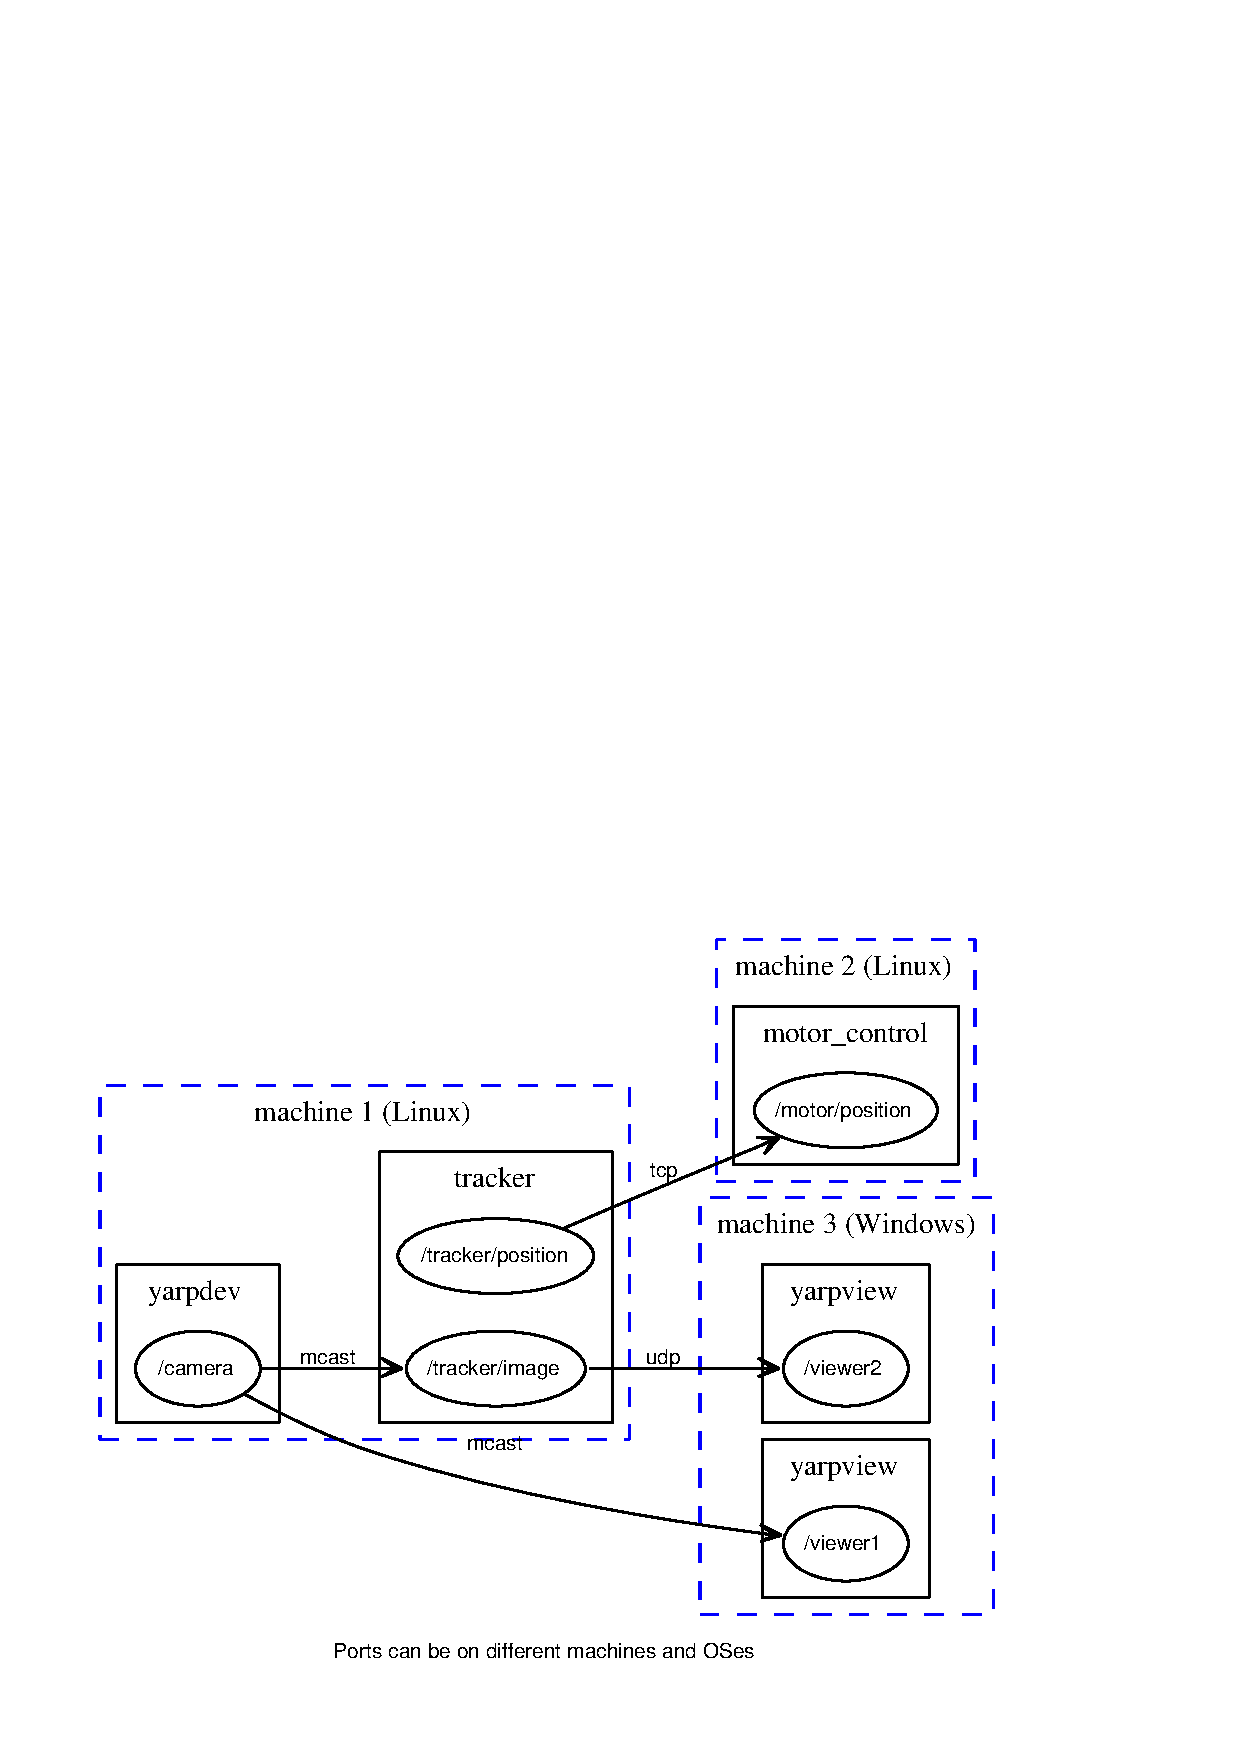
\includegraphics[width=10cm]{fig-ports}
}
\caption{
%
\label{fig:yarp-network}
%
Example of a network of ports.
Images are transmitted from a camera (``/camera'') port to a viewer
(``/viewer1'') port and the input of a visual tracker
(``/tracker/image''). The tracker annotates the image, for example by
placing a marker on a tracked point, and transmits that to another
viewer (``/viewer2''). The tracker also sends just the tracked position
from a position output port (``/tracker/position'') to a input
controlling head position (``/motor/position''). Every port belongs to a
process. They do not need to belong to the same process or 
be on the same machine as each other.  Every individual
connection can take place using a different protocol or physical
network~-- in the figure multicast, udp, and tcp are shown.
%
}
\end{figure}

For the purposes of YARP, communication takes place through
``connections'' between named entities called ``ports''. These form a
directed graph, the ``YARP Network'', where ports are the nodes, and
connections are the edges.
%
Each port is assigned a unique name, such as
``/icub/camera/left''. Every port is registered by name with a ``name
server''. The goal is to ensure that if you know the name of a port,
that is all you need in order to be able to communicate with it from
any machine.  The YARP name server (YNS) is a generalization of DNS
name service on the public internet for converting from domain names
to IP addresses.  It is not concerned just with machines but all
the details necessary to make a connection with a specific resource.
The YARP
name server is designed to be easily used by clients who are not
themselves using the YARP libraries or executables.  

The purpose of ports is to move data from one thread to another (or
several others) across process and machine boundaries. The flow of
data can be manipulated and monitored externally (e.g. from the
command-line) at run-time.  It can also be accessed without
using the YARP libraries or executables, since the relevant protocols
are documented.  If messages follow YARP guidelines, then they can be
automatically converted to and from a ``text mode'' connection, 
enabling human monitoring and intervention in the system,
and providing an easy way to experiment with integration with
non-YARP modules.

A port can send data to any number of other ports. A port can receive
data from any number of other ports. Connections between ports can be
freely added or removed, and may use different underlying transports.
The use of several different transports
and protocols allows us to exploit their best
characteristics.  TCP is reliable, it can be used to guarantee the
reception of a message.  UDP can be faster than TCP, but without
guarantees.  Multicast is efficient for distributing the same
information to large numbers of targets.  Shared memory can be
employed for local connections.  Text-mode operation is much
more human-friendly, and a good place to get started with
external integration.
Figure~\ref{fig:yarp-network} shows a very simple network of ports
for a visual tracking application.


%% The YARP name server is a server that tracks information about
%% ports. It indexes this information by name, playing a role analogous
%% to DNS on the internet. To communicate with a port, the properties of
%% that port need to be known (the machine it is running on, the socket
%% it is listening on, the carriers it supports). The YARP name server
%% offers a convenient place to store these properties, so that only the
%% name of the port is needed to recover them.


%% Upon creation, by default every port communicates with a server and is
%% allocated a ``contact'' (an abstract address).  By default this is a
%% free socket port number to listen on using tcp.  The port will make
%% itself available for communication as directed.  Its responsibility
%% is only to listen for communication, and upon receiving anything
%% to create its side of a connection (and then immediately return 
%% to listening).  This is simply a generalization of a server socket.


%%\subsection{Port abstraction}

Connections between ports in YARP can carry replies if desired
(and if the underlying protocol supports that), so
conventional ``RPC'' (remote procedure call) style synchronous
operation is possible.  We encourage streaming rather than RPC
whenever possible, because RPC can make a network brittle by
introducing strong coupling of timing between processes.
%
%%Connections can use different protocols.
%%Ports belong to processes.
%%Processes can be on different machines/OS.
%
%% We've separated out most of the plumbing.  We get to change it
%% dynamically (handy).  More importantly, we have better modularity.
%% Programs can be moved around as load and OS/device/library
%% dependencies dictate.  Fundamental protocol for communication can be
%% changed without affecting programs.  Better chance that your code can
%% be used by others (even just within your group).
%
For our implementation of ports, we have broken them down into 
several logically separable parts:

\begin{itemize} \pflist

\item The carrier factory (called ``Carriers'');
carrier is our generic name for any different transport or
protocol that can carry a connection.
  This factory maintains
a list of managers for different kinds of connection.  The user
can extend this list with their own custom types of connection
(for example, for a kind of network we've never considered,
or a different implementation of an existing carrier).


\item The core communications module (called ``Port'').  This
will manage connect requests, disconnects, reading, writing,
and various administrative details.  It defers to the carrier
factory to create specific connections and knows very little
about their nature.

\item Reader and writer buffers (called ``PortReaderBuffer'' and
``PortWriterBuffer'').  In order for communication to be efficient and
avoid unnecessary copies, objects being transmitted generally need to
be left untouched until communication is complete.  With the variety
of possible connections and options possible, the details of this can
become complicated.  YARP implements a certain set of policies we
think are good in the reader/writer buffer classes.  These are wrapped
around the Port class to provide a BufferedPort class that gives both
a simple interface and efficient implementation, while keeping
buffering and communication separable for those with strong opinions
about how one or the other should be done.

\item The YARP network interface (called ``Network'').  Provides
methods for manipulating parts of the network, such as
creating or removing connections between ports.

\end{itemize}

The YARP name server is a simple program using a single ordinary
port as its input; it used to have its own special protocol but
now it is just like any other YARP program.  This is possible 
because ports can operate without access to a name server if
desired; it is another separable component.

%, which was once a specially written server with
%its own protocol, is now written using a single ordinary port as its
%input.

%The flexibility of ports to maintain diverse kinds of connections
%simultaneously is 

%hidden from the user unless they want
%to do something very particular.  



\subsection{Human readable/writable communication}

There is a constant tension between using binary formats and
human-readable formats.  Binary formats can be much more efficient,
but text mode formats can be much easier to work with and learn about
experimentally without extensive study.  The value of text formats and
protocols has been seen time and time again in the short history of
computing (postscript, http, html, xml, etc.).

The YARP communications system is written in two parts.  The 
first part is  a set of ``carriers'' which do the work of providing
connections between ports, so that data can be faithfully 
transmitted from a source to a destination byte-for-byte.
There is no marshalling process at this stage.
%
The second part of the communication system is a standard data format.
This standard is specified separately 
from the carriers, so that the carriers could be reused by
someone with different opinions about data representation, but helper
functions and classes make it easy to meet.  This format is called the
``bottle'' format for historical reasons\footnote{
From YARP's online documentation:
{\it The name of this class comes from the idea of throwing a "message in a
bottle" into the network and hoping it will eventually wash ashore
somewhere else. In the very early days of YARP, that is what
communication felt like.}
}.  
There is a general-purpose
helper class in YARP called ``Bottle'' that reads and writes data in
this format, but the format is also used by special purpose classes
such as Vector and Image.  Extensive examples are available on how
to generate data in this form.
%
%% The bottle representation is based on a nested structure of certain
%% primitive types.  Here are some informal examples of bottles,
%% expressed in text form (an equivalent binary form can be used
%% interchangeably):
%
%% \begin{center}
%% \begin{tabular}{lp{6cm}}
%% \hline\hline
%% {\bf text-form bottle} & {\bf interpretation} \\
%% \hline
%% 10 20 30 & a list of three integers \\
%% 10.0 20.5 31.4159 & a list of three floating point numbers \\
%% action "go left" (10 20 30) & a list of two strings (``action'' and ``go left''), and a nested list of integers \\
%% {[set] [pos] 1 30.3} & a list of two vocabs, an integer, and a floating
%% point number -- perhaps to set the position of a specific axis. \\
%% \hline\hline
%% \end{tabular}
%% \end{center}
%
%% The structure is basically that of an s-expression
%% \cite{rivest1997sexp}, except that the outermost parentheses are
%% omitted.  This makes the important and common case of messages without
%% any nesting easier to write for those unfamiliar with s-expressions.
%% The drawback is that this means that a bottle must always be a list,
%% rather than any of the other primitive types, and (depending on the
%% input mechanism) it may also need to be non-empty.
%
The primitives types are simple and familiar:
 lists, integers, floating point
numbers, strings, blobs (uninterpreted sequence of bytes), and
``vocabs''.  The vocab type is the one unfamiliar type in this list.
It is motivated by the dual requirements of efficiency of machine
interpretation binary representations, and ease of human reading and
writing of text representations.  For data with a tag in it upon which
a dispatch will occur, it is simplest if that tag is a simple integer
in binary mode rather than a piece of variable-length text.
Vocabs are represented as simple integers in binary, and short
(up to four ASCII character) strings in text, with a one-to-one
mapping between the characters and bytes in the integer.  
%
%
The important point is that under normal operation, ports can be
sending fixed size messages to each other, but then when a human
eavesdrops on that data or tries to insert a message, they can still
understand and generate the identifiers being used.
%
%
The basic constraints on the design of this format were as follows:

\begin{itemize} \pflist

\item Messages in ths format should have a convenient binary and text
representation.

\item The process of translating between binary and text
representations should be mechanical, and ``round-trips'' should not
change the value significantly (except potentially with some round-off
in floating point numbers).

\item The text representation should be as easy as possible
to express from the command-line of common shells.

\end{itemize}

The reason for the last item is to make YARP messaging compatible
with typical UNIX pipe operation.  Such operation does not 
really survive well when different character encodings may be
in use, but still has uses.


Bottle-style messages
can be expressed in several interchangeable representations:
binary, text, command-line options, configuration
files etc.  
%
We find that under various conditions sometimes we want the same kind
of data coming from file, command line options, or across the network,
so is convenient to have all the various representions mapping to a
homogeneous structure.
%% For messaging there are:

%% \begin{itemize} \pflist

%% \item Binary form -- used for efficient messaging that is
%% easily machine readable/writable.

%% \item Text form -- used for messaging that is easily human
%% readable/writable (but less efficient for large messages).

%% \end{itemize}

%% It is also convenient to add two extra representations:

%% \begin{itemize} \pflist

%% \item Command-line form -- arguments to a program.

%% \item Configuration form -- groups and lines in a configuration file.

%% \end{itemize}

%% \subsection{Examples}

%% Capital letters are constants
%% (L=List, D=Double, I=Integer, S=String, B=Blob, V=Vocab).

%% A vector of 4 doubles.  S-expression: (1.0 -20.0 76.2 41.9).

%% \newcommand{\mm}{p{0.25cm}}
%% \newcommand{\m}{p{1cm}}
%% \newcommand{\md}{p{2cm}}

%% \begin{tabular}{|\m|\m|\md|\md|\md|\md|}
%% \hline
%% L+D & 4 & 1.0 & -20.0 & 76.2 & 41.9 \\
%% \hline
%% \end{tabular}


%%\subsection{Fiddling with the format}

%For robotics applications that are confined to a 
%local area network with all source code available,
%changes to the data format are possible.

%% The default binary representation for integers on
%% the wire for YARP is little-endian.  Conversions
%% happen for non big-endian systems (e.g. MAC PPC).
%% For a network that is all big-endian,  the 
%% binary representation can be flipped. 

%% This could also be desired for XDR compatibility.
%% The string and blob representations also would
%% need to be updated to do padding which YARP does
%% not do.  These changes would be very narrowly
%% localized.

%% Such a modified system would lose binary-mode compatibility with any
%% modules using the standard YARP binary format, but connections could
%% still be made in text mode.

In principle, evolution of the communication protocol in YARP can be
relatively painless.  Since new ``carriers'' can be added,
modifications could be placed within a new carrier, while support for
older carriers is continued for a generation or two.  Ideally,
something like today's text mode format should be honored for a long
time, as a connection protocol of last resort.

%%(NOTE: this is about more than just the bottle format; reorder).


\subsection{Connection protocol}

This is the protocol used for a single connection from an output port
to an input port. It has two main phases, the handshake phase,
and the message phase.
%
We begin once the sender has successfully opened a bidirectional
streaming connection (think: tcp socket) to the receiver.
First comes the {\bf handshake phase}:

\begin{itemize} \pflist

\item {\bf Transmission of protocol specifier}:
Sender transmits 8 bytes that identify the ``carrier'' that will be
used for the connection.  The carrier can require switching to 
some other form of stream, or using a particular strategy for
encoding data.  The transmission of the initial 8 bytes is the
only part of this protocol that is defined in terms of bytes sent.

\item {\bf Transmission of sender name}: Sender transmits the name of
the port it is associated with.  How this name is encoded and sent is
the concern of the specific carrier.

\item {\bf Transmission of extra header material}: Sender and
receiver may engage in further communication as needed for the
specific carrier.  

\end{itemize}

At the end of this phase, the sender and receiver are both ``aware''
of which carrier is in use (this may have involved discarding the
original stream and switching to a new one -- e.g. mcast, udp, shared
memory) and both are aware of the identifier of the port at the
other end of the connection.  This can be important for collaboration
during connection shutdown.


Next comes the {\bf message phase}.
After the handshake, the connection is (as far as YARP is concerned)
quiescent until either the sender decides to send a message across it.
It is technically possible for the receiver to initiate activity --
we'll return to this issue.

\begin{itemize} \pflist

\item {\bf Transmission of index}: Carrier-dependent. Some carriers
will require statistics about the message (such as its length) to be
given at the beginning.  YARP binary carriers have a fairly elaborate
index, due historically to a limitation of the QNX message-passing
API.  Text-mode carriers have no index at all, since it is
unreasonable to expect a human to be able to generate one.

\item {\bf Transmission of payload}: The actual message is
transmitted in a carrier-dependent way.

\item {\bf Acknowledgement of payload}: The receiver may 
acknowledge transmission in some way.  Carrier-dependent.

\end{itemize}

The message phase repeats as often as the user wants.
%
The description so far sounds very loose -- just about every aspect
of a connection is carrier-dependent.  What does YARP actually
expect of connections, in order to build on them?

\begin{itemize} \pflist

\item After the handshaking phase, both sides of a connection know the
names of the other side.  This is important for housekeeping.

\item After the handshaking phase, a connection endpoint must have
certain knowledge about the connection that it can report to YARP.  It
will be connection-based or connectionless.  It will be text mode or
binary.  It will deliver acknowledgements or not.  It will be able to
deliver replies or not.  It will be active or ``fake'' (in multicast,
many logical connections can be serviced with a single active
connection -- these details are taken care of at the carrier level).

\end{itemize}

%% Before sending each message, YARP also expects the endpoint to know
%% whether the connection can be ``escaped'' -- that is, it can accept
%% port-to-port administrative communication that is not passed on as
%% normal user data.  The only time escaping is not desired on a carrier
%% is in text-mode, when the bytes transmitted should follow the user
%% data as slavishly as possible.  In all other cases, some
%% administrative data is currently packaged by YARP with user data and
%% then extracted at the other end.  In future carriers will be given
%% more control over how this material (called the ``port protocol'') is
%% embedded.


\begin{table}
\begin{center}
\begin{tabular}{ll}
\hline
\hline
{\bf 8-byte magic number}&{\bf protocol} \\\hline
`Y' `A' 0xE4 0x1E 0 0 `R' `P'&tcp \\
`Y' `A' 0x61 0x1E 0 0 `R' `P'&udp\\
`Y' `A' 0x62 0x1E 0 0 `R' `P'&multicast\\
`Y' `A' 0x63 0x1E 0 0 `R' `P'&shared memory\\
`C' `O' `N' `N' `E' `C' `T' `\textvisiblespace' &text \\
`C' `O' `N' `N' `A' `C' `K' `\textvisiblespace' &text-with-ack \\
`G' `E' `T' `\textvisiblespace' `/' \ldots &http\\
  \ldots & \ldots\\\hline\hline
\end{tabular}
\end{center}
\caption{
%
Partial list of YARP connection ``magic numbers'' -- the eight initial
bytes of a connection in YARP specify the desired protocol to use from
that point on.  Magic numbers are commonly used in all sorts of file
formats intended for interchange.
YARP's rather strange magic numbers for binary formats (``YAnnnnRP'')
evolved in order to be compatible with earlier versions of itself.
%
}
\end{table}

The important point about the communication protocol is that
is {\em polymorphic} and allows {\em heterogeneous} use --
the protocol on each connection between two ports can be 
controlled independently.  This allows for system evolution,
where new protocols are introduced, potentially mapping onto
radically different physical networks, virtual networks,
or external middleware.


\subsection{YARP without YARP}

Suppose some YARP programs are running and we want to send or
receive data from them.
%
For example, suppose there is a YARP system running, with a 
port called ``/motors'' which will accept commands to move a
motor.  For concreteness, let's imagine we have started the
following standard YARP programs (on the same or different 
machines):

\begin{verbatim}
yarp server
yarpdev --device test_motor --axes 2 --single_port --name /motors
\end{verbatim}

The ``yarpdev'' program here creates a port called ``/motors'' that can
accept command to a fake set of motors (2 axes or degrees of freedom),
and report on their state.
%
Normally we would interact with the motor through a code
interface that deals with communication.  But if for 
some reason we can't use the YARP codebase, what can
we do?

YARP ports listen to incoming tcp connections, always ready to make
new connections for input or output.  Suppose we can discover that
``/motors'' is listening on port 10022 of our current machine (we could
discover that using netstat on Linux, or by querying the YARP server
as we'll see shortly).
%
We can then connect manually to the port as follows:

\begin{center}
\begin{tabular}{ll}
\hline\hline
{\bf user types} & {\bf system responds} \\
\hline
{\bf \$} telnet 127.0.0.1 10022 & {\it (telnet startup message)} \\
CONNECT foo & Welcome foo \\
help & {\it (an explanation of available commands)} \\
* & This is /demo at tcp://127.0.0.1:10032 ... \\
\hline\hline
\end{tabular}
\end{center}

Everything so far would be basically the same for any YARP port.
For people who have used MUDs, IRC, or serial interfaces to hardware,
it should all seem vaguely familiar.
%
So far all our communications have been ``administrative'' --
we have communicated with the port but not really with the 
program that owns it.  To do that, we send payload data.  For the
text-mode carrier we've chosen (determined by the 8 initial
bytes we sent, ``CONNECT '' in this case), this is done by typing
``d'', hitting return, then writing a text-mode representation of
the data we want to send.  Let's try it:

\begin{center}
\begin{tabular}{ll}
\hline\hline
{\bf user types} & {\bf system responds} \\
\hline
 d & {\it (no response, waiting for data)} \\
 help & {\it (a list of available yarpdev commands)} \\
 d & {\it (no response, waiting for data)} \\
 {[get] [axes]} &  {[is] [axes] 2 [ok]} \\
 d & {\it (no response, waiting for data)} \\
 {[set] [pos] 0 100.0} & {[ok]} \\
\hline\hline
\end{tabular}
\end{center}

We have determined that there are indeed two axes available as we requested
when starting yarpdev, and have set the position target for the
first axis to 100.0 units.  We could go on to query positions, use
other interfaces, etc.  We can disconnect by closing our connection
(or, more politely, sending the message ``q'').

By default, the motor port will stream encoder readings from the motors
to any reader that connects.  To subscribe to this stream, we simply
connect as above and then type ``r'' to reverse the connection.
Reversing means to invert which side should take the initiative
in sending data.


\begin{center}
\begin{tabular}{ll}
\hline\hline
{\bf user types} & {\bf system responds} \\
\hline
{\bf \$} telnet 127.0.0.1 10022 & {\it (telnet startup message)} \\
CONNECT foo & Welcome foo \\
r & do \\
& 100.0 0.0 \\
 & do \\
 & 100.0 0.0 \\
 & {\it (continues streaming motor state)} \\
 & \ldots \\
\hline\hline
\end{tabular}
\end{center}


The ``do'' is just like ``d'', to inform the recipient that user data
follows (as opposed to an administrative message).  
The ``o'' part means that replies are not expected by the
sender, and should not be sent.  This seems like a small detail,
but in fact when replies are not expected the performance of 
streaming to multiple targets can be greatly improved in general,
so it is worth mentioning.

Suppose we wanted to send messages more efficiently?  We start out the
same way, connecting via TCP, and then give the ``magic number'' of
the carrier we want to use (tcp binary, udp, mcast, shmem, etc).
Understanding these carriers is a bit harder than basic text-mode operation,
but logically it is all the same thing.

One part we skipped at the start was how to discover how to 
access ports in ths first place.  If we know the port we want
is called ``/motors'', how do we discover where it is?  We can
in fact talk to the yarp name server using exactly the same 
protocol that we have described here.

%% To do that, we need to talk to the ``yarp server'', which is analogous
%% to a standard DNS name server.  If we're using YARP, our program would
%% be able to discover where the server is by itself (by checking
%% standard configuration files if available or sending broadcast
%% messages if necessary).  Or, if we don't want to use yarp at all, we
%% can simply make a note of what machine and port number it is running
%% on.  Suppose it is on 127.0.0.1 listening to port number 10000.
%% We can communicate with the name server exactly as with any regular
%% port.


%% \begin{center}
%% \begin{tabular}{lp{8cm}}
%% \hline\hline
%% {\bf user types} & {\bf system responds} \\
%% \hline
%% {\bf \$} telnet 127.0.0.1 10000 & {\it (telnet startup message)} \\
%% CONNECT foo & Welcome foo \\
%%  d & {\it (no response, waiting for data)} \\
%%  help & {\it (a list of available name server commands)} \\
%%  d & {\it (no response, waiting for data)} \\
%%  {query /motors} &  registration name /motors ip 127.0.0.1 port 10022 type tcp \\
%% \hline\hline
%% \end{tabular}
%% \end{center}


%% So we now know how to reach /motors (tcp connection to 127.0.0.1 port 10022).
%

So, with a running YARP system, we can to discover
and communicate with running programs, sending commands and reading
data, without using any YARP libraries or executables.  All the steps
we've gone through are trivial in any language with a basic socket
library (we're not using any special features of telnet, it is just
for demonstration purposes).  It is important to remember, though,
that while we've been communicating with the ``/motors'' port using
text across tcp, at the same time the same port could be communicating
with other programs via binary messages over udp or multicast etc.
%
We believe the existence of the bottle format for communicating
with YARP processes makes it much easier to experiment with and build
bridges to in text-mode (like http for the web), while gracefully
supporting switching to binary-mode communication when the 
situation demands it.

%What if we wanted to make a port ourselves?  To make a full-featured
%port supporting all the carriers that YARP does would be quite a lot
%of work.  To make a basic port that just supports text-mode tcp
%communication is easier.  A demo is a little cumbersome for this paper...

